\documentclass{article}

\usepackage[czech]{babel}
\usepackage{amsmath,amsfonts}
\usepackage[utf8]{inputenc}
%\usepackage[T1]{fontenc}
%\usepackage{czech}
\usepackage[unicode]{hyperref}
\usepackage{epsfig}
\usepackage{indentfirst}	% Odsazení prvního odstavce

\author{Pavel Stránský}
\title{Kratičké seznámení se s \LaTeX em}

\frenchspacing				% Mezery mezi slovy a mezi větami stejné
\pagestyle{headings}

\def\uv#1{\clqq{#1}\crqq}	% Makro pro české uvozovky

\begin{document}
	\maketitle
	
	\section{Odstavce}	
	\label{sec:odstavce}
	Pro odsazení prvního odstavce je nutné použít balík \textbf{indentfirst}.

	Nezáleží,      kolik
	mezer      vkládáme       ve zdrojovém
	textu
	mezi     slova.
	
	Nový odstavec se vloží pomocí prázdného řádku.
	
	Řádky v dlouhém odstavci se automaticky zalomí. 
	Řádky v dlouhém odstavci se automaticky zalomí. 
	Řádky v dlouhém odstavci se automaticky zalomí. 
	Řádky v dlouhém odstavci se automaticky zalomí. 
	Řádky v dlouhém odstavci se automaticky zalomí. 
	
	\LaTeX{} automaticky dělí slova.
	\LaTeX{} automaticky dělí slova.
	\LaTeX{} automaticky dělí slova.
	\LaTeX{} automaticky dělí slova.
	\LaTeX{} automaticky dělí slova.
	
	Po jednopísmenných předložkách a spojkách dáváme nedělitelné mezery pomocí symbolu~\~{}.
	Rovněž například mezi den a měsíc u data.
	Vypadá to líp.
	
	\section{Uvozovky}
	Různé druhy uvozovek: \uv{české} (vytvořené pomocí makra) nebo ``English''.

	\section{Pomlčky}
	Půjde-li to, sejdeme se v 10--16~hodin.
	Důležité je, abychom v textu --- to je to, co teď píšeme --- správně používali pomlčky.
	V anglickém jazyce se používají trochu jinak než v českém.
	
	\section{Výpustky}
	To máte cihly, hřebíky, šrouby, matky, vruty, \ldots

	\section{Háčky, čárky a další ozdůbky}
	\label{sec:akcenty}
	H\^otel,
	na\"\i ve, 
	\'el\`eve, 
	sm\o rrebr\o d, 
	!‘Se\~norita!,	
	Sch\"onbrunner Schlo\ss stra\ss e,
	pot\r u\v cek
	
	\`a \'a \^a \r a \v a \"a  \H a
	\~a \=a \b a \.a \u a \t{aa} \c a \d a
	
	\section{Nadpisy}
		Důležité je nejen, jak text vypadá, ale i jak je strukturovaný.
	\subsection{Podsekce}
	\subsubsection{Podpodsekce}
	\paragraph{Odstavec}
	\subparagraph{Pododstavec}	
	
	\section{Křížové odkazy}
	V sekci~\ref{sec:akcenty} na straně~\pageref{sec:akcenty} jsou příklady veškeré diakritiky, kterou~\LaTeX{} zná.
	Rovnice~\eqref{eq:Brouncker} se mi obzvlášť líbí.
	
	\section{Poznámky pod čarou}
	Poznámka pod čarou\footnote{V některých stylech ani čára nemusí být přítomna} se píší velmi jednoduše.
	
	\section{Zvýraznění textu a různá písma}
	\emph{Důležité myšlenky} je potřeba zvýraznit.
	
	\section{Výčty}
	Výčty mohou být buď
	\begin{enumerate}
		\item číslované
	\end{enumerate}
	nebo
	\begin{itemize}
		\item nečíslované.
	\end{itemize}
	
	\section{Rovnice}
	V textu se zapisují pomocí znaku dolaru: $a^2+b^2=c^2$.
	Na speciální řádku se hodí složitější rovnice, jako je třeba Leibnizova řada pro výpočet čísla $\pi$:
	\begin{equation}
		\frac{\pi}{4}=\sum_{k=1}^{\infty}\frac{(-1)^{k+1}}{2k-1}
			=1-\frac{1}{3}+\frac{1}{5}-\dotsb
	\end{equation}
	
	Pro číslo $\pi$ existují i jiné formule, třeba tato Newtonova
	\begin{equation}
		\pi=\frac{3}{4}\sqrt{3}+24\int_{0}^{\frac{1}{4}}\sqrt{x-x^2}dx,
	\end{equation}
	Vietova --- nekonečný součin vnořených odmocnin
	\begin{equation}
		\frac{2}{\pi}=\sqrt{\frac{1}{2}}\sqrt{\frac{1}{2}+\frac{1}{2}\sqrt{\frac{1}{2}}}\sqrt{\frac{1}{2}+\frac{1}{2}\sqrt{\frac{1}{2}+\frac{1}{2}\sqrt{\frac{1}{2}}}}\dotsb
	\end{equation}
	nebo Brounckerova pomocí řetězových zlomků
	\begin{equation}
		\label{eq:Brouncker}
		\frac{4}{\pi}=1+\frac{1^2}{2+\frac{3^2}{2+\frac{5^2}{2+\frac{7^2}{2+\dotsb}}}}
	\end{equation}
	
	Mezery je v matematických textech potřeba ošetřit zvlášť:
	\begin{equation}
		\forall x\in\mathbb{R}\qquad x^{2}\geq0 \quad\textrm{(platí skoro vždy)}
	\end{equation}
	
	Jelikož proměnné se sází kurzívou, zatímco názvy funkcí nikoliv,
	jsou v \LaTeX u speciální příkazy pro funkce:
	\begin{equation}
		\sin^{2}x+\cos^2{x}=1
	\end{equation}
	
	Velikost závorek je nejlepší nechat přímo na \LaTeX u:
	\begin{equation}
		f(x)=\left[\sum_{n=1}^{\infty}\frac{\left(x^2-1\right)^n}{n}\right]^2
	\end{equation}
	
	Pro všemožné symboly je dobré konzultovat bohaté zdroje na webu,
	například několikasetstránkový dokument~\cite{ref:SymbolList}. 
	
	\section{Obrázky}
	Obrázky se doporučuje používat jako plovoucí objekty, což znamená, že se neobjeví přesně tam, kde je vložíme, nýbrž tam, kam nejlépe padnou a kde splní všechna typografická pravidla.
		\begin{figure}[!htbp]
			\centering
			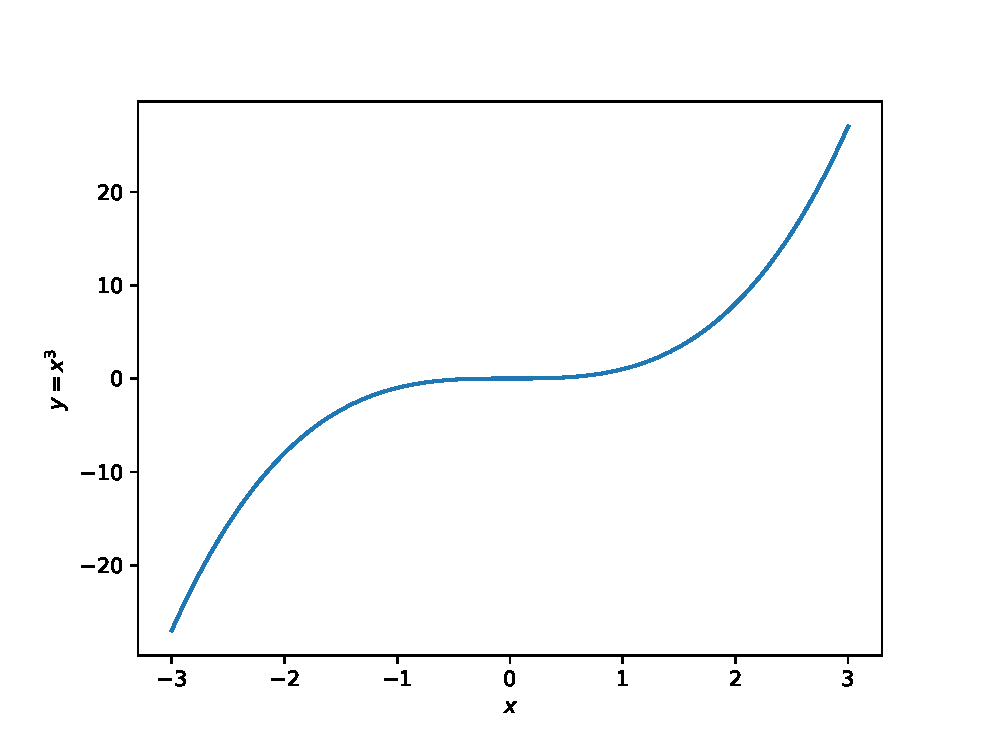
\includegraphics[width=0.8\linewidth]{kubik.eps}
			\caption{Kubická funkce $y=x^3$.}
			\label{fig:bandf}
		\end{figure}	

	\section{Závěr}
		K úplně základnímu seznámení se s psaním v \LaTeX u tento text může stačit.
		Rozhodně doporučuji přečíst si nějaký trochu podrobnější návod, jakým je například~\cite{ref:UvodLaTeX}.

	\begin{thebibliography}{99}
		\bibitem{ref:SymbolList} S. Pakin, \href{http://tug.ctan.org/info/symbols/comprehensive/symbols-a4.pdf}{The comprehensive \LaTeX{} Symbol List} (2017).
		\bibitem{ref:UvodLaTeX} T. Oetiker, H, Partl, I. Hyna, E. Schlegl, M. Kočer, P. Sýkora,
			\href{http://www.penguin.cz/~kocer/texty/lshort2e/lshort2e-cz.pdf}{Ne příliš stručný návod do systému \LaTeXe} (1998).
	\end{thebibliography}

	\tableofcontents

\end{document}
